\documentclass[../main.tex]{subfiles}
\begin{document}
%=========================================================
% TĐ_GiaoAn_IQA_HK1_Tuan16_CacSoTrongPhamVi100_SoTronChuc
% Giáo án Toán tư duy cấp độ A - Chủ đề CÁC SỐ TRONG PHẠM VI 100. SỐ TRÒN CHỤC
% (Buổi 1, Buổi 2) - bản biên soạn lại: tăng trò chơi, câu hỏi gợi mở, phân hóa HS
% Soạn theo mẫu (\hktuan, \subsection, hd, vd, luuy)
% Hình đặt trong thư mục Hinh_GiaoAn_Tuan16/ (cùng cấp với file này), tên hình có tiền tố ga16_
\graphicspath{{Hinh_GiaoAn_Tuan16/}{Data_GiaoAn_HK0/Hinh_GiaoAn_Tuan16/}}
%=========================================================

%---------- Lệnh dùng riêng cho giáo án ----------
% Chèn hình căn giữa, dính liền với đoạn phía trên; tham số = chiều cao tối đa
\providecommand{\TThinh}{}\renewcommand{\TThinh}[2][8cm]{\par\nopagebreak\vspace{2pt}\nopagebreak{\centering\includegraphics[height=#1,width=\linewidth,keepaspectratio]{#2}\par}\vspace{2pt}}
% Chỗ chấm điền
\providecommand{\TTcham}[1][3cm]{\makebox[#1]{\dotfill}}
% Tiêu đề mục nhỏ trong một hoạt động
\providecommand{\GAmucnho}{}\renewcommand{\GAmucnho}[1]{\par\addvspace{4pt}\noindent{\color{mauchinh}\bfseries #1}\par\nopagebreak\addvspace{2pt}}
% Lời GV nói với HS (in nghiêng, có dấu ngoặc kép)
\providecommand{\GAloi}{}\renewcommand{\GAloi}[1]{\textit{“#1”}}
% Bó que tính và que lẻ: \GAbo{n}, \GAle{n}
\providecommand{\GAbo}{}\renewcommand{\GAbo}[1]{\foreach \i in {1,...,#1}{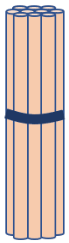
\includegraphics[height=1.5cm]{ga16_image11.png}\hspace{1pt}}}
\providecommand{\GAle}{}\renewcommand{\GAle}[1]{\foreach \i in {1,...,#1}{
\includegraphics[height=1.5cm]{ga16_image12.png}\hspace{3pt}}}
% Dãy ô số: \GAday{a,b,,d,...} (để trống = ô trống)
\providecommand{\GAday}{}\renewcommand{\GAday}[1]{%
  \begin{tikzpicture}\foreach \x [count=\k] in {#1}{\node[draw,thick,minimum width=1.05cm,minimum height=0.8cm,font=\large] at (1.05*\k,0) {\x};}\end{tikzpicture}}

%%%%%%%%%%%%%%%%%%%%%%%%%%%%%%%%%%%%%%%%%%%%%%%%%%%%%%%%%%
%                       BUỔI 1
%%%%%%%%%%%%%%%%%%%%%%%%%%%%%%%%%%%%%%%%%%%%%%%%%%%%%%%%%%
%\setcounter{section}{3} % không chỉnh sửa
\hktuan{1}{16}
\par\medskip
%\textbf{Người soạn: }
\begin{center}
        {\color{mauchinh!120}\bfseries\Large CÁC SỐ TRONG PHẠM VI 100. SỐ TRÒN CHỤC (BUỔI 1)}
\end{center}

\subsection{MỤC TIÊU CẦN ĐẠT}
\begin{itemize}
    \item \textbf{Kiến thức:} HS đếm, đọc, viết được các số trong phạm vi 100; đếm tới, đếm lùi.
    \item \textbf{Kiến thức:} HS nhận biết hàng chục, hàng đơn vị của số có hai chữ số (1 chục = 10 đơn vị).
    \item \textbf{Kiến thức:} HS nhận biết số tròn chục (10, 20, \dots, 90) và đếm được theo chục.
    \item \textbf{Năng lực:} HS mạnh dạn trả lời, biết hợp tác trong nhóm 2 -- 3 bạn.
    \item \textbf{Phẩm chất:} HS hào hứng, tự tin, biết chờ lượt và cổ vũ bạn.
\end{itemize}

\subsection{TIẾN TRÌNH DẠY HỌC}
\textbf{Đồ dùng dạy học:} giáo án, PBT, bút, khăn ẩm, laptop/TV, con dấu, sticker ngôi sao, bó que tính (mỗi bó 10 que, có dây buộc), bảng con, thẻ số từ 1 đến 100, bảng số 1 -- 100 in khổ lớn (có ô trống).

\begin{luuy}
    \textbf{Cách tính điểm cả buổi:} mỗi nhóm có một “cây ngôi sao” trên bảng. Trả lời đúng, làm nhanh, hợp tác tốt đều được dán sao. Cuối buổi nhóm nhiều sao nhất được tặng sticker và được chọn bài hát khởi động cho buổi sau.
\end{luuy}

%---------------------------------------------------------
\subsubsection{KHỞI ĐỘNG -- SỬA BÀI TẬP VỀ NHÀ}
\begin{hd}
    \begin{itemize}
        \item Thời gian: 15 phút
        \item Tạo không khí vui, ổn định lớp; sửa BTVN và ôn đếm trong phạm vi 20.
    \end{itemize}
\end{hd}
\GAmucnho{Trò chơi “Chuyền bóng đếm số” (5 phút)}
\begin{itemize}
    \item Cả lớp đứng thành vòng tròn (hoặc ngồi tại chỗ). GV tung quả bóng nhỏ và nói một số, ví dụ \GAloi{15}. Bạn bắt bóng nói số liền sau (16) rồi chuyền cho bạn khác.
    \item Khi GV vỗ tay 2 cái, cả lớp đổi chiều: đếm \textbf{lùi}. Bạn nào nói sai thì làm một động tác vui (nhảy lò cò, làm mặt cười) rồi chơi tiếp, không bị loại.
\end{itemize}
\GAmucnho{Sửa BTVN: “Thám tử tìm lỗi” (10 phút)}
\begin{itemize}
    \item GV chọn 2 -- 3 bài làm có lỗi sai thường gặp (che tên HS), chiếu lên TV và hỏi: \GAloi{Thám tử nào tìm ra lỗi sai?}
    \item HS giơ tay chỉ lỗi và giải thích cách sửa. GV khen ngợi cả bạn tìm ra lỗi lẫn tinh thần dũng cảm sửa sai.
\end{itemize}

%---------------------------------------------------------
\subsubsection{TRÒ CHƠI “GIẢI CỨU BẢNG SỐ”}
\begin{hd}
    \begin{itemize}
        \item Thời gian: 20 phút
        \item HS đọc, viết, sắp xếp được các số từ 1 đến 100; nhận ra quy luật của bảng số.
    \end{itemize}
\end{hd}
\begin{itemize}
    \item \textbf{Câu chuyện dẫn dắt:} \GAloi{Bạn Gió tinh nghịch vừa thổi bay mất nhiều số trong bảng số của lớp mình. Các đội hãy giải cứu và đưa các số về đúng nhà nhé!}
    \item GV chia nhóm 2 -- 3 HS, phát bảng số 1 -- 100 có ô trống và thẻ số. Nhóm nào điền đúng và nhanh nhất được 3 sao, nhóm nhì 2 sao, các nhóm còn lại hoàn thành được 1 sao.
    \item Sau khi chơi, GV hỏi để HS tự phát hiện quy luật:
    \begin{itemize}
        \item[--] \GAloi{Đi sang phải một ô thì số thay đổi thế nào?} (thêm 1)
        \item[--] \GAloi{Đi xuống một ô thì sao?} (thêm 10, chữ số hàng chục tăng 1)
        \item[--] \GAloi{Cột cuối cùng có gì đặc biệt?} (toàn số tròn chục: 10, 20, \dots, 100)
    \end{itemize}
\end{itemize}
\begin{center}
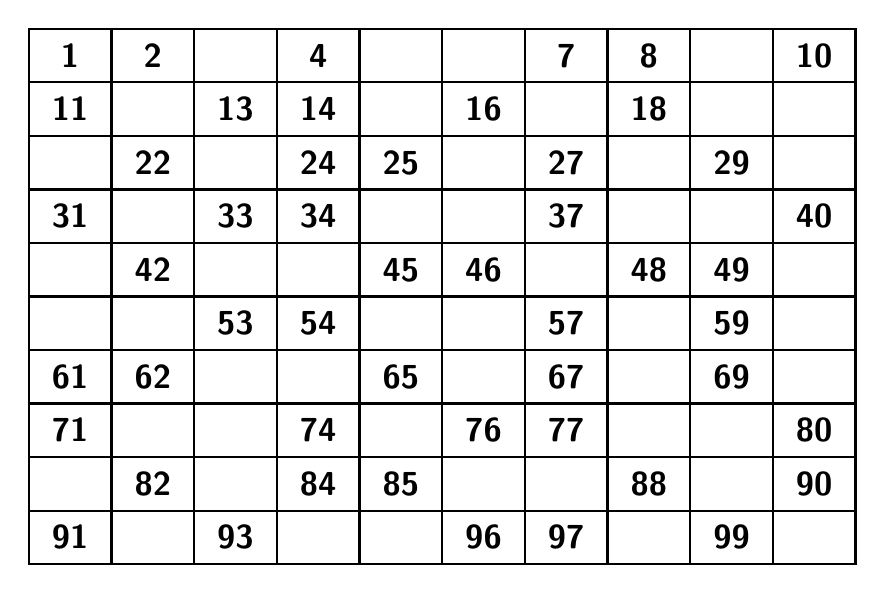
\begin{tikzpicture}[font=\sffamily\bfseries\large]
    \foreach \hang [count=\i] in {{1,2,,4,,,7,8,,10},{11,,13,14,,16,,18,,},{,22,,24,25,,27,,29,},{31,,33,34,,,37,,,40},{,42,,,45,46,,48,49,},
                                  {,,53,54,,,57,,59,},{61,62,,,65,,67,,69,},{71,,,74,,76,77,,,80},{,82,,84,85,,,88,,90},{91,,93,,,96,97,,99,}}{
        \foreach \so [count=\j] in \hang{\node[draw,thick,minimum width=1.05cm,minimum height=0.68cm] at (1.05*\j,-0.68*\i) {\so};}}
\end{tikzpicture}
\end{center}
\begin{luuy}
    Phân hóa: nhóm HS chậm được phát thêm “thẻ gợi ý” (dãy số của hàng đó); nhóm HS nhanh được thử thách thêm: \GAloi{Tìm tất cả số có chữ số 5 ở hàng đơn vị.}
\end{luuy}
\GAmucnho{Luyện tập trong PBT: Bài 1, Bài 2}
\textbf{Bài 1.} Hãy đếm số vật trong các hình dưới đây và điền đáp số vào ô trống. \textit{(Gợi ý cho HS: đếm theo từng hàng 10 rồi đếm tiếp phần lẻ.)}
\par\nopagebreak\vspace{2pt}
{\centering
    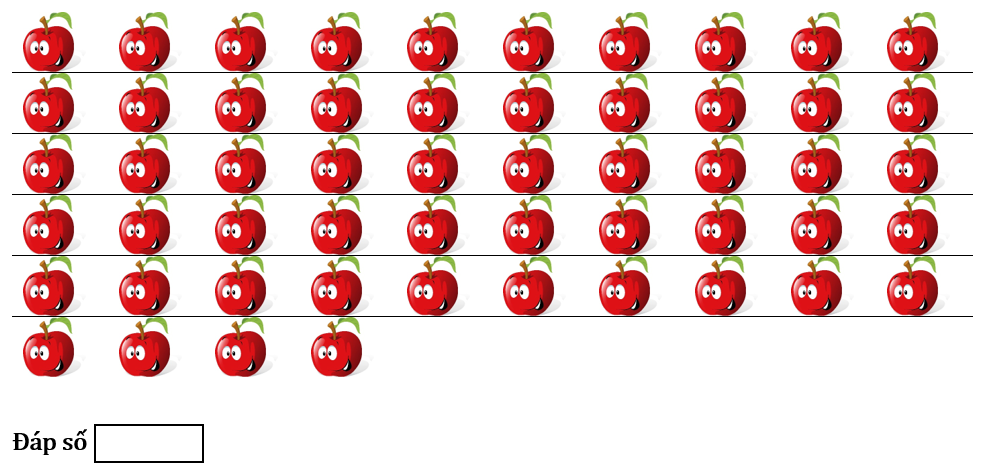
\includegraphics[width=0.48\linewidth]{ga16_image2.png}\hfill
    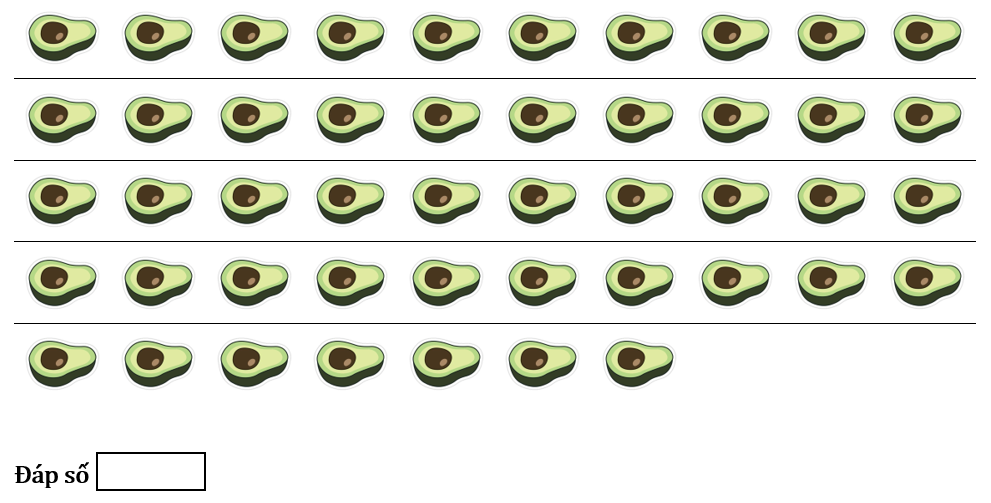
\includegraphics[width=0.48\linewidth]{ga16_image3.png}\\[4pt]
    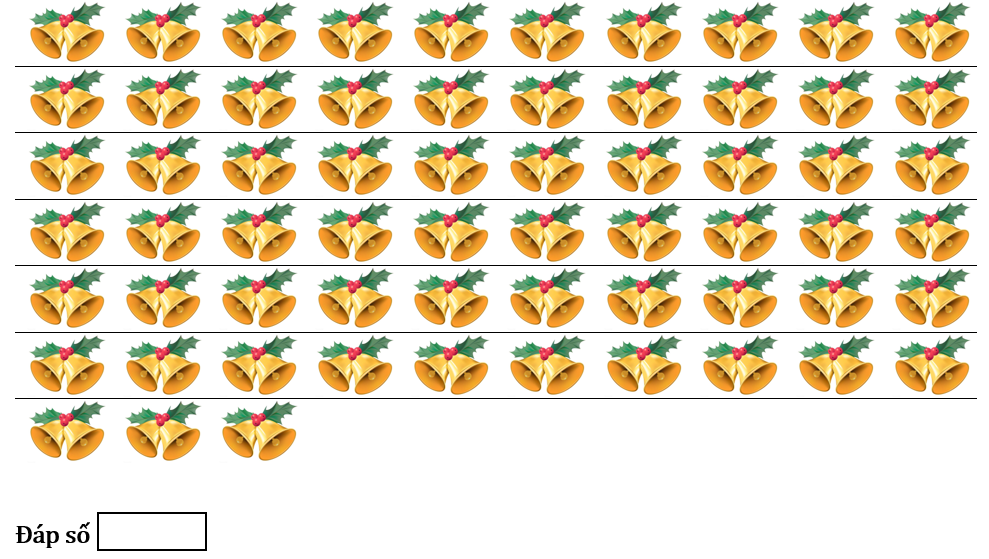
\includegraphics[width=0.48\linewidth]{ga16_image4.png}\hfill
    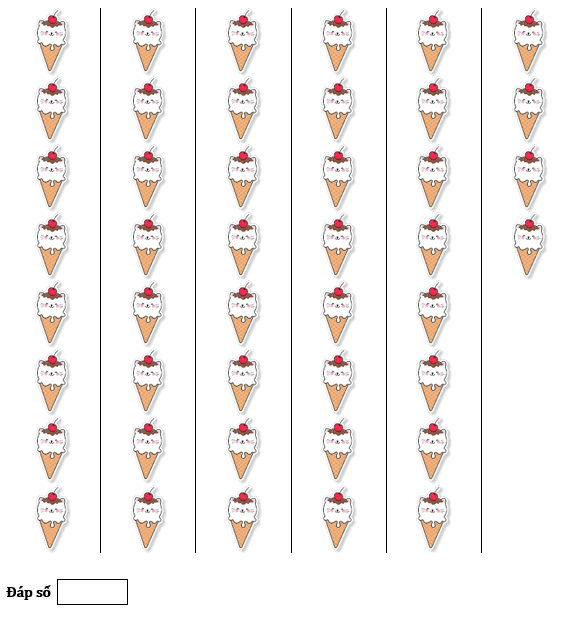
\includegraphics[height=4.6cm]{ga16_image5.png}\par}
\medskip
\textbf{Bài 2.} Nối với số thích hợp.
\TThinh[6cm]{ga16_image6.png}

%---------------------------------------------------------
\subsubsection{TRÒ CHƠI “ĐOÀN TÀU ĐẾM SỐ”}
\begin{hd}
    \begin{itemize}
        \item Thời gian: 5 phút
        \item HS đếm tới, đếm lùi nhanh và chính xác trong phạm vi 100.
    \end{itemize}
\end{hd}
\begin{itemize}
    \item Cả lớp làm “đoàn tàu”: mỗi bạn là một toa, lần lượt nói một số. GV là “trưởng tàu” hô: \GAloi{Tàu chạy tới từ 21!} -- HS đếm 21, 22, \dots, 26 rồi quay lại 21, 22, \dots
    \item GV hô \GAloi{Tàu lùi!} -- đoàn tàu đổi sang đếm lùi 26, 25, \dots, 21. Toa nào nói đúng được 1 sao cho nhóm.
    \item Tăng dần độ khó: đổi phạm vi (48 -- 53, 67 -- 72), đổi chiều nhanh hơn, hoặc cho “tàu tốc hành” đếm thật nhanh.
\end{itemize}

%---------------------------------------------------------
\subsubsection{CẤU TẠO SỐ -- “SIÊU THỊ QUE TÍNH”}
\begin{hd}
    \begin{itemize}
        \item Thời gian: 20 phút
        \item HS hiểu 1 chục = 10 đơn vị; tách được số có hai chữ số thành chục và đơn vị; đọc, viết đúng.
    \end{itemize}
\end{hd}
\GAmucnho{a) Khám phá: 10 que thành 1 bó}
\begin{itemize}
    \item GV phát cho mỗi nhóm một nắm que lẻ và hỏi: \GAloi{Đếm từng que rất lâu, làm sao đếm nhanh hơn?} Gợi ý HS gom đủ 10 que buộc thành 1 bó.
    \item GV giơ 1 bó que và chốt: \textbf{1 que là 1 đơn vị; 1 bó que (10 que) là 1 chục. 1 chục = 10 đơn vị.}
\end{itemize}
\begin{center}
    \GAbo{1}\quad\raisebox{0.6cm}{\Large $=$}\quad\GAle{10}
\end{center}
\GAmucnho{b) “Siêu thị que tính”}
\begin{itemize}
    \item GV đóng vai người bán hàng: \GAloi{Cô cần mua 32 que tính, bạn nào lấy giúp cô?} HS lấy 3 bó và 2 que lẻ, vừa lấy vừa đếm: \GAloi{mười, hai mươi, ba mươi, ba mươi mốt, ba mươi hai}.
    \item GV hỏi: \GAloi{3 bó là mấy chục? 2 que lẻ là mấy đơn vị?} và ghi vào bảng:
\end{itemize}
\begin{center}
    \renewcommand{\arraystretch}{1.3}
    \begin{tabular}{|>{\centering\arraybackslash}m{4.2cm}|>{\centering\arraybackslash}m{2.8cm}|>{\centering\arraybackslash}m{2.4cm}|>{\centering\arraybackslash}m{3.2cm}|}
        \hline
        \textbf{Hàng chục} & \textbf{Hàng đơn vị} & \textbf{Viết số} & \textbf{Đọc số} \\ \hline
        \GAbo{3} & \GAle{2} & & \\
        3 & 2 & 32 & Ba mươi hai \\ \hline
    \end{tabular}
\end{center}
\begin{itemize}
    \item GV đổi vai cho HS làm “người bán hàng”, các bạn khác lấy que theo yêu cầu (45, 58, 70, \dots).
    \item Trò chơi nhanh \textbf{“Ai giơ bảng nhanh nhất”}: GV giơ số bó và số que lẻ, HS viết số lên bảng con.
\end{itemize}
\begin{luuy}
    Lỗi HS hay gặp, GV chú ý sửa ngay:
    \begin{itemize}
        \item Viết “ba mươi hai” thành 302 (viết cả 30 và 2) $\Rightarrow$ cho HS đặt que vào bảng chục -- đơn vị để thấy chỉ có 2 chữ số.
        \item Đọc 25 là “hai mươi năm”, 21 là “hai mươi một” $\Rightarrow$ đọc đúng: \textbf{hai mươi lăm, hai mươi mốt}; 24 đọc “hai mươi bốn” hoặc “hai mươi tư”.
        \item Nhầm 23 và 32 $\Rightarrow$ hỏi lại: \GAloi{Chữ số nào chỉ số bó que?}
    \end{itemize}
\end{luuy}
\GAmucnho{Luyện tập trong PBT: Bài 3, Bài 4}
\textbf{Bài 3.} Viết số tương ứng với số lượng que tính.
\par\nopagebreak\vspace{2pt}
{\centering
    \renewcommand{\arraystretch}{1.15}
    \begin{tabular}{|>{\centering\arraybackslash}m{6.2cm}|>{\centering\arraybackslash}m{5.2cm}|>{\centering\arraybackslash}m{2.6cm}|}
        \hline
        \GAbo{4} & \GAle{4} & \textbf{44} \\ \hline
        \GAbo{6} & \GAle{6} & \\ \hline
        \GAbo{3} & \GAle{9} & \\ \hline
        \GAbo{7} & \GAle{4} & \\ \hline
        \GAbo{8} & \GAle{9} & \\ \hline
        \GAbo{6} & \GAle{6} & \\ \hline
        \GAbo{9} & \GAle{2} & \\ \hline
    \end{tabular}\par}
\medskip
\textbf{Bài 4.} Điền số thích hợp vào chỗ trống.
\par\nopagebreak\vspace{2pt}
{\centering
    \renewcommand{\arraystretch}{1.5}
    \begin{tabular}{|>{\centering\arraybackslash}p{2.2cm}|>{\centering\arraybackslash}p{2.8cm}|>{\centering\arraybackslash}p{2.8cm}|>{\centering\arraybackslash}p{5cm}|}
        \hline
        \textbf{Số} & \textbf{Hàng chục} & \textbf{Hàng đơn vị} & \textbf{Cách đọc} \\ \hline
        43 & & & \\ \hline
         & 5 & 7 & \\ \hline
         & & & Bảy mươi sáu \\ \hline
        98 & & & \\ \hline
        27 & & & \\ \hline
         & & & Sáu mươi chín \\ \hline
         & 7 & 2 & \\ \hline
    \end{tabular}\par}

%---------------------------------------------------------
\subsubsection{SỐ TRÒN CHỤC -- “TÒA NHÀ SỐ TRÒN CHỤC”}
\begin{hd}
    \begin{itemize}
        \item Thời gian: 20 phút
        \item HS nhận biết số tròn chục là số có chữ số hàng đơn vị bằng 0; đếm tới, đếm lùi theo chục.
    \end{itemize}
\end{hd}
\begin{itemize}
    \item GV giơ lần lượt 1, 2, 3, \dots bó que (không có que lẻ) và hỏi: \GAloi{Có mấy chục que? Viết số nào?} HS phát hiện: \GAloi{Không có que lẻ nên hàng đơn vị là 0.}
    \item GV chốt: \textbf{Số tròn chục là số có chữ số hàng đơn vị bằng 0.}
    \item GV vẽ “tòa nhà” 10 tầng trên bảng, mỗi tầng là một số tròn chục. HS lên dán thẻ số vào đúng tầng.
\end{itemize}
\begin{center}
    \renewcommand{\arraystretch}{1.6}
    \begin{tabular}{|*{5}{>{\centering\arraybackslash}p{2.6cm}|}}
        \hline
        \textbf{1 chục = 10} & \textbf{2 chục = 20} & \textbf{3 chục = 30} & \textbf{4 chục = 40} & \textbf{5 chục = 50} \\ \hline
        \textbf{6 chục = 60} & \textbf{7 chục = 70} & \textbf{8 chục = 80} & \textbf{9 chục = 90} & \textbf{10 chục = 100} \\ \hline
    \end{tabular}
\end{center}
\GAmucnho{Trò chơi “Vỗ tay số tròn chục”}
\begin{itemize}
    \item GV đọc một dãy số bất kì: 18, 20, 35, 40, 41, 70, 99, 100, \dots Gặp số tròn chục, cả lớp vỗ tay 2 cái và hô “Tròn chục!”; gặp số khác thì ngồi im.
    \item Đếm tới, đếm lùi theo chục bằng cách “leo cầu thang”: đứng lên một bậc khi đếm tới (10, 20, \dots, 100), ngồi xuống một bậc khi đếm lùi (100, 90, \dots, 10).
\end{itemize}
\begin{vd}
    Điền số tròn chục còn thiếu:
    \par\nopagebreak\vspace{4pt}{\centering\GAday{10,20,,40,,,70,,90,}\par}
\end{vd}

%---------------------------------------------------------
\subsubsection{CỦNG CỐ -- GIAO BÀI TẬP VỀ NHÀ}
\begin{hd}
    \begin{itemize}
        \item Thời gian: 10 phút
        \item HS tự tổng kết bài học; GV đánh giá nhanh mức độ hiểu bài.
    \end{itemize}
\end{hd}
\begin{itemize}
    \item \textbf{“Vé ra về”:} mỗi HS nhận một mẩu giấy nhỏ, viết: (1) một số tròn chục em thích; (2) số 47 gồm mấy chục, mấy đơn vị. Bạn nộp vé đúng được đóng dấu “Ngôi sao hôm nay”.
    \item GV đếm sao, tuyên dương nhóm thắng cuộc và các bạn tiến bộ.
    \item GV giao BTVN phù hợp với tình hình lớp.
\end{itemize}

%%%%%%%%%%%%%%%%%%%%%%%%%%%%%%%%%%%%%%%%%%%%%%%%%%%%%%%%%%
%                       BUỔI 2
%%%%%%%%%%%%%%%%%%%%%%%%%%%%%%%%%%%%%%%%%%%%%%%%%%%%%%%%%%
\newpage
\setcounter{subsection}{0}
\begin{center}
        {\color{mauchinh!120}\bfseries\Large CÁC SỐ TRONG PHẠM VI 100. SỐ TRÒN CHỤC (BUỔI 2)}
\end{center}

\subsection{MỤC TIÊU CẦN ĐẠT}
\begin{itemize}
    \item \textbf{Kiến thức:} HS ôn lại cách đếm số và cấu tạo số có hai chữ số.
    \item \textbf{Kiến thức:} HS đếm được theo cách 2, cách 5, cách 10.
    \item \textbf{Kiến thức:} HS cộng, trừ được các số tròn chục.
    \item \textbf{Năng lực:} HS quan sát, phát hiện quy luật dãy số; trình bày cách làm trước lớp.
    \item \textbf{Phẩm chất:} HS tích cực tham gia trò chơi, trung thực khi tự kiểm tra kết quả.
\end{itemize}

\subsection{TIẾN TRÌNH DẠY HỌC}
\textbf{Đồ dùng dạy học:} giáo án, PBT, bút, khăn ẩm, laptop/TV, con dấu, sticker, bó que tính, bảng con, chuông nhỏ, thẻ số.

%---------------------------------------------------------
\subsubsection{KHỞI ĐỘNG -- “RUNG CHUÔNG VÀNG MINI”}
\begin{hd}
    \begin{itemize}
        \item Thời gian: 15 phút
        \item Ổn định lớp; kiểm tra nhanh kiến thức buổi 1 (đọc, viết, cấu tạo số trong phạm vi 100).
    \end{itemize}
\end{hd}
\begin{itemize}
    \item Mỗi HS một bảng con. GV đọc 5 câu, HS viết đáp án và giơ bảng khi nghe tiếng chuông. Bạn trả lời đúng cả 5 câu được nhận “huy hiệu chuông vàng”.
\end{itemize}
\begin{vd}
    Câu hỏi gợi ý:
    \begin{multicols}{2}
    \begin{enumerate}
        \item Viết số “sáu mươi tư”. \hfill (64)
        \item Số 58 gồm mấy chục, mấy đơn vị? \hfill (5 chục, 8 đơn vị)
        \item Số liền sau của 39 là số nào? \hfill (40)
        \item Viết một số tròn chục lớn hơn 60. \hfill (70, 80, 90)
        \item Số liền trước của 100? \hfill (99)
    \end{enumerate}
    \end{multicols}
\end{vd}

%---------------------------------------------------------
\subsubsection{ÔN TẬP -- “ĐOÁN SỐ BÍ MẬT”}
\begin{hd}
    \begin{itemize}
        \item Thời gian: 15 phút
        \item HS đếm nhanh theo chục; phân tích được chữ số hàng chục, hàng đơn vị.
    \end{itemize}
\end{hd}
\begin{itemize}
    \item GV chiếu (hoặc giơ) một số bó que và que lẻ trong 3 giây rồi che lại: \GAloi{Số bí mật là số mấy?}
    \item Sau khi HS trả lời (ví dụ 42), GV hỏi tiếp: \GAloi{Chữ số 4 ở hàng nào? Chữ số 2 ở hàng nào? 42 gồm mấy chục mấy đơn vị? Số liền trước, liền sau của 42?}
    \item Đổi vai: một HS nghĩ số bí mật và gợi ý \GAloi{Số của tớ có 6 chục và 3 đơn vị}, cả lớp đoán.
\end{itemize}
\begin{center}
    \GAbo{4}\quad\GAle{2}\quad\raisebox{0.55cm}{\Large $\rightarrow$ 42}
\end{center}

%---------------------------------------------------------
\subsubsection{ĐẾM CÁCH 2, CÁCH 5, CÁCH 10 -- “VŨ ĐIỆU ĐẾM SỐ”}
\begin{hd}
    \begin{itemize}
        \item Thời gian: 30 phút
        \item HS đếm được theo cách 2, cách 5, cách 10 trong phạm vi 100 và vận dụng để đếm nhanh đồ vật.
    \end{itemize}
\end{hd}
\begin{itemize}
    \item GV nhắc lại đếm cách 2 đã học trong phạm vi 20: 0, 2, 4, 6, \dots, 20; tăng dần lên đến 100.
    \item Mỗi cách đếm đi kèm một động tác để HS vừa đếm vừa vận động:
    \begin{itemize}
        \item[--] \textbf{Cách 2:} vỗ tay mỗi lần đếm (2, 4, 6, \dots). Gợi ý: đếm đôi đũa, đôi dép, đôi tất.
        \item[--] \textbf{Cách 5:} giơ một bàn tay 5 ngón (5, 10, 15, \dots). Gợi ý: đếm ngón tay của cả nhóm.
        \item[--] \textbf{Cách 10:} giơ cả hai bàn tay hoặc giơ một bó que (10, 20, 30, \dots).
    \end{itemize}
    \item Thi đua theo nhóm: nhóm nào đếm đúng nhịp, đồng đều nhất được 2 sao.
    \item GV cho HS đếm cách 2 ở các bài tập trong sách TiTan, sau đó làm Bài 1 trong PBT.
\end{itemize}
\GAmucnho{Luyện tập trong PBT: Bài 1. Đếm theo yêu cầu và điền kết quả}
\begin{listEX}
    \item Có bao nhiêu chiếc lá? Đếm cách 5.
    \TThinh[2.8cm]{ga16_image15.png}
    \item Có bao nhiêu hộp quà? Đếm cách 2.
    \TThinh[3.2cm]{ga16_image16.png}
    \item Có bao nhiêu cánh hoa? Đếm cách 5.
    \TThinh[3.2cm]{ga16_image17.png}
    \item Có bao nhiêu chùm nho? Đếm cách 10.
    \TThinh[2.4cm]{ga16_image18.png}
\end{listEX}
\begin{luuy}
    HS chậm: cho dùng que tính hoặc khoanh từng nhóm 2, 5, 10 trên hình rồi mới đếm. HS nhanh: đếm lùi cách 10 từ 100, hoặc đếm cách 5 bắt đầu từ 3 (3, 8, 13, \dots).
\end{luuy}

%---------------------------------------------------------
\subsubsection{TRÒ CHƠI “TÌM CON SỐ BÍ ẨN”}
\begin{hd}
    \begin{itemize}
        \item Thời gian: 10 phút
        \item HS phát hiện quy luật dãy số (thêm 1, thêm 2, thêm 5, thêm 10) và điền số còn thiếu.
    \end{itemize}
\end{hd}
\begin{itemize}
    \item GV phát phiếu cho từng cặp bạn cùng bàn. Cặp nào xong nhanh và đúng nhất được lên bảng làm “thầy/cô giáo nhỏ” chữa bài cho lớp.
    \item Trước khi điền, HS phải nói được “bí mật” của dãy số: \GAloi{Mỗi ô thêm mấy?}
\end{itemize}
\begin{center}
    \GAday{,32,33,,,,37,,,40}\\[6pt]
    \GAday{10,12,,,,,20}\\[6pt]
    \GAday{,10,15,,,,,40,}\\[6pt]
    \GAday{,10,20,,,50,}
\end{center}

%---------------------------------------------------------
\subsubsection{CỘNG, TRỪ CÁC SỐ TRÒN CHỤC}
\begin{hd}
    \begin{itemize}
        \item Thời gian: 15 phút
        \item HS cộng, trừ được các số tròn chục bằng cách nhẩm theo chục và bằng cách đặt tính.
    \end{itemize}
\end{hd}
\begin{itemize}
    \item \textbf{Nhẩm bằng que tính:} GV giơ 5 bó que, thêm 3 bó: \GAloi{5 chục thêm 3 chục là mấy chục?} $\Rightarrow$ 8 chục = 80. Vậy $50 + 30 = 80$.
    \item \textbf{Đặt tính:} GV nhắc HS viết các chữ số thẳng cột (hàng đơn vị thẳng hàng đơn vị, hàng chục thẳng hàng chục), tính từ phải sang trái.
\end{itemize}
\begin{center}
    \Large
    $\begin{array}{r@{\,}r}
        & 50\\
      + & 30\\ \hline
        & 80
    \end{array}$
    \qquad\qquad
    $\begin{array}{r@{\,}r}
        & 70\\
      - & 40\\ \hline
        & 30
    \end{array}$
\end{center}
\begin{itemize}
    \item \textbf{Trò chơi “Tiếp sức”:} chia lớp 2 đội; GV ghi các phép tính cộng, trừ số tròn chục trên bảng. Từng bạn lên làm một phép tính rồi chạy về đập tay bạn tiếp theo. Đội xong trước và đúng nhiều hơn thắng.
    \item GV chốt mẹo nhẩm nhanh: \textbf{chỉ cộng (trừ) các chữ số hàng chục, giữ nguyên chữ số 0 ở hàng đơn vị}.
    \item GV cho HS làm bài tập vận dụng trong sách TiTan.
\end{itemize}
\begin{vd}
    $20 + 40 = 60$ \qquad $60 + 30 = 90$ \qquad $80 - 50 = 30$ \qquad $90 - 60 = 30$
\end{vd}

%---------------------------------------------------------
\subsubsection{CỦNG CỐ -- GIAO BÀI TẬP VỀ NHÀ}
\begin{hd}
    \begin{itemize}
        \item Thời gian: 10 phút
        \item HS nhắc lại kiến thức trọng tâm; GV nhận xét, khen thưởng.
    \end{itemize}
\end{hd}
\begin{itemize}
    \item \textbf{“Hộp quà bí mật”:} chuyền hộp quà theo nhạc, nhạc dừng ở bạn nào thì bạn đó bốc một câu hỏi trong hộp (đếm cách 2 từ 40 đến 50; đếm lùi cách 10 từ 90; $30 + 20 = ?$, \dots).
    \item GV ôn tập lại đếm tới, đếm lùi, đếm cách 2, 5, 10; tuyên dương nhóm nhiều sao nhất và các bạn tiến bộ.
    \item GV giao BTVN phù hợp với HS lớp mình.
\end{itemize}

\begin{center}
       \faGg\faGg\quad Hết \quad\faGg\faGg
\end{center}
\end{document}
